\draft Scattering structure factor.

Sketch of the direct lattice:
\begin{figure}[H]
	\centering
	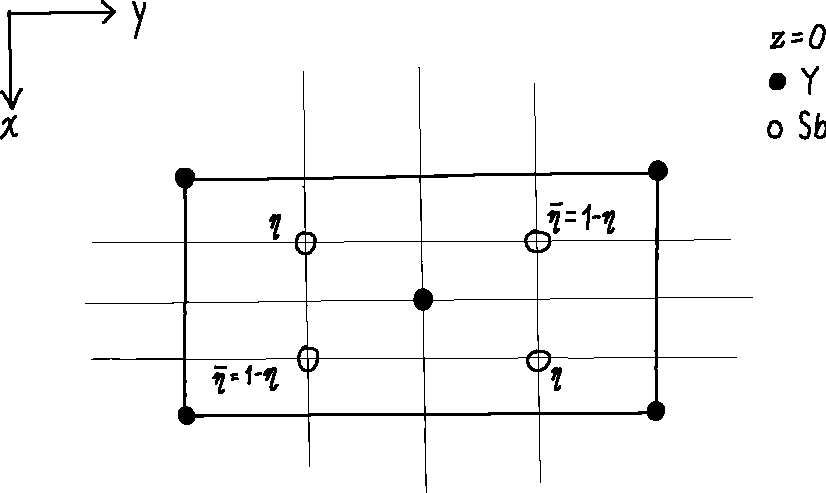
\includegraphics[width=.6\linewidth]{q1-direct-lattice}
\end{figure}

\begin{parts}
	\part Scattering amplitude for reciprocal lattice vector $\mathbf{G} = h\mathbf{a}^* + k\mathbf{b}^*$ + l$\mathbf{c}^*$ and C-centred lattice with centering translation $(\diagfrac{1}{2}, \diagfrac{1}{2}, 0)$:
	\begin{align*}
		S_{hkl} &= f_x \sbracket{\mathrm{e}^{i0} + \mathrm{e}^{2\pi i\rbracket{h \cdot 1/2 + k \cdot 1/2 + 0}}} \\
		&= f_x \rbracket{1 + \mathrm{e}^{\pi i\rbracket{h+k}}}
	\end{align*}
	where $f_x$ is the atomic factor for atom $x$ (assumed to be common throughout the lattice points).
	
	So extinction condition is when $S_{hkl} = 0$ $\Rightarrow$ $h+k=$ odd.
	
	\part
	\begin{figure}[H]
		\centering
		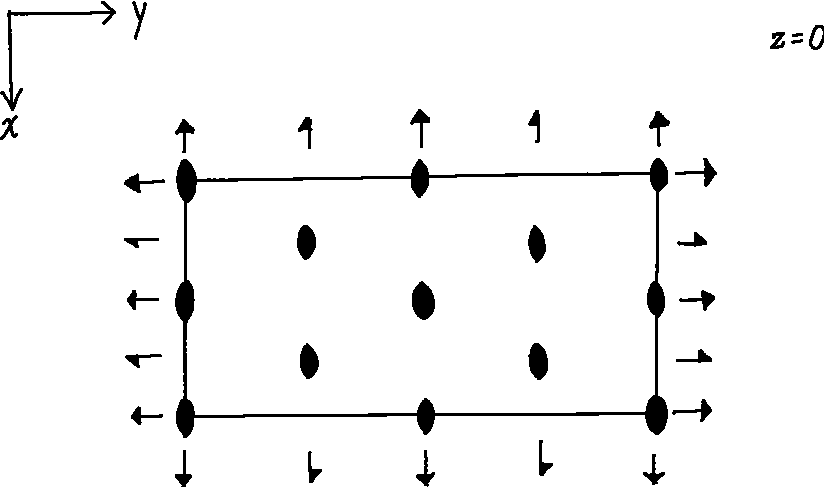
\includegraphics[width=.6\linewidth]{q1-symmetry-elements}
	\end{figure}
	As seen above, there is no point of inversion.
	Nor are there any mirror planes.
	However, there exists screw axis of $2_1$ as pointed by the half-pointed arrows in the diagram above.
	
	\part Generally,
	\begin{align*}
		S_{hkl} &= S_\textnormal{basis} \times S_\textnormal{lattice} \\
		&= \rbracket{1 + \mathrm{e}^{i\pi\rbracket{h+k}}} \sbracket{f_\textnormal{Y} \mathrm{e}^{i0} + f_\textnormal{Sb} \rbracket{\mathrm{e}^{2\pi i\rbracket{h/4 + k/4 + l\eta}} + \mathrm{e}^{2\pi i\rbracket{3h/4 + k/4 - l\eta}}}} \\
		&= \rbracket{1 + \mathrm{e}^{i\pi\rbracket{h+k}}} \sbracket{f_\textnormal{Y} + f_\textnormal{Sb}\rbracket{\mathrm{e}^{2\pi i\rbracket{h/4 + k/4 + l\eta}} + \mathrm{e}^{2\pi i\rbracket{-h/4 + k/4 - l\eta}}}} \\
		&= \ldots\sbracket{f_\textnormal{Y} + f_\textnormal{Sb} \mathrm{e}^{i\pi k/2} \cdot 2\cos\rbracket{h/2 + 2l\eta}\pi} \\
		&= 2 \times \begin{cases}
			f_\textnormal{Y} + f_\textnormal{Sb} \rbracket{-1}^{k/2} \cdot 2\cos\rbracket{h/2 + 2l\eta}\pi \qquad \textnormal{$h$, $k$ even} \\
			f_\textnormal{Y} + f_\textnormal{Sb} i^{k/2} \cdot 2\cos\rbracket{h/2 + 2l\eta}\pi \qquad \textnormal{$h$, $k$ odd}
		\end{cases}
	\end{align*}
	
	\part Note that enantiomorphs have opposite signs for $\eta$, so the extinction condition for either would have a phase difference of $4l\eta$.
	By comparing between the calculations for $\pm\eta$ and the scattering angle, we may distinguish between the 2 forms.
	
	\part Note that shearing has destroyed the 2-fold rotational symmetry along $x$ and $y$.
	However the 2 along $z$ and C centering is preserved, so we have a monoclinic C121 lattice.
\end{parts}